% kapitel2.tex
\chapter{Grundlagen}
\label{chapter: kap2}

\section{Machine Learnings Grundbegriffe}
\label{section: Basics}
Bei künstlicher Intelligenz handelt es sich um einen Teilbereich der Informatik, doch eine genaue, allgemeine Definition gibt es nicht. Der Begriff wird oft für bestimmte Szenarien beschrieben. Dabei überschneidet sich ein entscheidender Teil: Es werden Computer entwickelt, die in der Lage sind, sich menschenähnlich zu verhalten. Dieses schließt zum Beispiel die Fähigkeit zu Lernen oder zur Selbstverbesserung ein \cite{} \Todo{Referenzen}{} und ermöglicht es intelligenten Systemen, Entscheidungen zu treffen. Oftmals sind diese Klassifizierungen für Menschen schwierig zu entscheiden oder zu erkennen oder sehr komplex.

Doch es ist nicht nur der allgemeine Oberbegriff, der nicht allgemeingültig ist. Auch viele andere Bezeichnungen sind austauschbar oder unterschiedlich definiert, abhängig von einem speziellen Problem. Andere Begrifflichkeiten sind dagegen allgemein etabliert. Im folgenden werden die in dieser Arbeit verwendeten Benennungen und entsprechende Synonyme zur Klarheit definiert.

\begin{definition}
	\label{def: KI}
	Künstliche Intelligenz (KI), intelligente Systeme
	
	Die Bezeichnungen Künstliche Intelligenz und intelligentes System werden austauschbar verwendet und bezeichnen in dieser Arbeit Computer, die sich menschenähnlich verhalten können \cite{}.
\end{definition}

\begin{definition}
	\label{def: ML}
	Machine Learning (ML, maschninelles Lernen)
	
	Mit dem Begriff Machine Learning wird der gesamte Lernprozess für ein intelligentes System bezeichnet. Dieser beinhaltet mehrere verschiedene Schritte, die abhängig von bestimmten Problemstellungen in ihrer konkreten Realisierung variieren können. Er Beschreibt das Entwerfen eines Algorithmus, der das gegebene Problem akkurat löst \cite{Basics-ML, Basics-ML2, Basics-ML-Blog}.
\end{definition}

Die Grundlage für maschinelles Lernen bilden jedoch immer Daten, deren Art (Bilder, Texte, Tonaufzeichnungen, etc.) und Anzahl sowie die Menge und Vielfalt der einzelnen vorhanden Feature können vollkommen unterschiedlich sein. Auf diesen werden dann verschiedenste Berechnungen ausgeführt. Heutzutage handelt es sich dabei oft um verschiedene Netze (wie zum Beispiel in \ref{section: NN} beschrieben).

Im Allgemeinen gibt es für bestimmte Probleme mehrere Optionen, einen festgelegten Algorithmus mithilfe von Parametern zu modifizieren, sodass die vorgegebene Berechnung möglichst gut an die Daten angepasst ist. 

\begin{definition}
	\label{def: Training}
	Training/ Lernen / Lernprozess
	
	Eine künstliche Intelligenz wird trainiert, wenn die Parameter eines Algorithmus verändert werden, sodass die Ausgabe des Netzes (siehe \ref{section: NN}) schrittweise verbessert und an die Datengrundlage angepasst wird. \cite{Basics-ML-Blog} \Todo{Referenzen}{}
	Eine genauere Erläuterung des Lernprozesses ist in Kapitel \ref{section: Lernprozess} angegeben.
\end{definition}

Ein Datenpunkt ist hierbei ein einzelnes Objekt aus allen vorhanden Daten, die für das Training, oder das Testen einer Funktion verwendet werden. Dabei wird entsprechend zwischen Trainings- und Testdaten unterschieden. \cite{} \Todo{Referenzen}{} Ein Trainingsdatum wird zum Trainieren, also im Lernprozess eines Netzes (siehe Kapitel \ref{section: NN}) verwendet,  \cite{Basics-Training-Daten-ehler-CrossValidation} ein Testbeispiel zum Testen der erlernten Klassifikationen genutzt. Bei letzteren handelt es sich um für das Netz noch unbekannte Daten, die dazu dienen, die Genauigkeit der Vorhersagen eines Netzes zu bestimmen. \cite{Basics-Training-Daten-ehler-CrossValidation} 
Eine Eigenschaft oder ein Feature beschreibt bestimmte Werte eines konkreten Datenpunktes. Für das \glqq Objekt\grqq einer Person können Eigenschaften zum Beispiel der Name, das Geschlecht oder das Alter sein. \cite{} \Todo{Referenzen}{}	

Neben den vielen Unterschieden in Definition und Verwendung bestimmter Begriffe haben sich jedoch einige allgemein durchgesetzt. Zu diesen gehören grundlegende Konzepte wie supervised und unsupervised (und semi-supervised learning) und die Unterscheidung in Klassifizierungs- und Regressionsprobleme. Letztere basiert zum Teil auf der vielen maschinellen Entscheidungen zugrundeliegenden Statistik und der Unterscheidung von Eigenschaften in qualitative und quantitative Merkmale.

\begin{definition}
	\label{def: Qualitativ}
	Qualitative Merkmale
	
	Eine Eigenschaft ist qualitativ, wenn sie nominalskaliert (durch einen Begriff beschrieben) oder ordinalskaliert (durch Ziffern beschrieben, jedoch ohne Aussage über eine Größe der Abstände). Auf diesen Werten kann in der Regel nicht sinnvoll gerechnet werden, da sie keine einheitlichen Skalen und/oder Abstände einhalten. Des weiteren sind qualitative Merkmale immer diskret. \cite{Basics-Statistik-Cramer, Basics-Statistik-Sachs}
	
	Typische Beispiele sind Namen, das Geschlecht oder Schulnoten. Name und Geschlecht sind dabei nominalskaliert, Schulnoten ordnial.
\end{definition}

\begin{definition}
	\label{def: Quantitiv}
	Quantitative / metrische Merkmale
	
	Ein quantitatives Feature lässt sich durch Zahlen angeben. Die Werte können sowohl diskret als auch stetig sein, ermöglichen aber in jedem Fall sinnvolle Rechnungen. Abstände sind auf diesen Merkmalen fest durch bestimmte Einheiten (z.B. durch die Einheit 1 für natürliche Zahlen) vorgegeben. \cite{Basics-Statistik-Cramer, Basics-Statistik-Sachs}
	
	Hierzu zählen zum Beispiel die Größe, das Alter oder andere Messungen, wie die Temperatur.
\end{definition}

Auf dieser Unterscheidung basiert die Differenzierung in Regressions- und Klassifizierungsprobleme. Hierbei ist jedoch die Ausgabe (siehe Definition \ref{def: Ausgabe}) entscheidend. 

\begin{definition}
	\label{def: Regression}
	Regressionsprobleme
	
	Handelt es sich bei der Ausgabe maschinellen Lernverfahrens um ein quantitives Merkmal, liegt ein Regressionsproblem vor. \cite{ISLRBuch}
\end{definition}

\begin{definition}
	\label{def: Klassifikation}
	Klassifikationsprobleme
	
	Gibt ein maschinelles Lernverfahren ein qualitatives Merkmal aus, handelt es sich um ein Klassifikationsproblem. \cite{ISLRBuch}
\end{definition}

Neben der Unterscheidung aufgrund der Ausgabeart eines Algorithmus wird auch die grundlegende Art des Lernens unterschieden in supervised, unsupervised und semi-supervised learning.

\begin{definition}
	\label{def: Supervised}
	Supervised Learning / überwachtes Lernen
	
	Beim Supervised Learning sind alle Trainingsdaten Klassifiziert. Die Ausgabe, die vom Algorithmus errechnet werden soll steht fest. Anhand dieses vorgegebenen korrekten Outputs kann somit das Ergebnis automatisch geprüft und eine Fehlerrate bestimmt werden. \cite{Basics-(un/semi)supervised}
	
	Zum Beispiel würde folgendes Szenario als supervised Learning kategorisiert werden:
	
	Die vorhandenen Daten sind Personendaten, anhand derer Kreditwürdigkeit bestimmt wurde. Alle Personendaten wurden bereits beurteilt (Kredit erhalten/ Kredit nicht erhalten) und sind mit den entsprechenden korrekten Labeln versehen. 
	Ein intelligentes System wird trainiert und lernt, Vorhersagen zu machen. Die Genauigkeit der Vorhersagen kann über die Fehlerrate anhand der anders klassifizierten Beispiele bestimmt werden. 
\end{definition}

\begin{definition}
	\label{def: Unsupervised}
	Unsupervised Learning / unüberwachtes Lernen
	
	Beim Unsupervised Learning sind die vorhandenen Trainingsdaten nicht vorher klassifiziert. Der Algorithmus teilt sie lediglich anhand verschiedener Kriterien in bestimmte Gruppen ein und gibt diese Gruppierung aus. Hierbei gibt es oft keine \glqq korrekten \grqq Antworten, da die zugrundeliegenden Daten keine besondere Einordnung enthalten. \cite{Basics-(un/semi)supervised}
	
	Zu unsupervised Learning gehört beispielsweise die Bestimmung von Ähnlichkeiten verschiedener User um Vorschläge (Filme, Produkte, etc.) zu generieren, die an die einzelnen Personen angepasst sind. Hierbei können die Nutzer nicht von vornherein in bestimmte Gruppen klassifiziert werden und eine Fehlerberechnung anhand falscher Ausgaben ist ebenfalls nicht möglich.
\end{definition}

\begin{definition}
	\label{def: Semi-Supervised}
	Semi-Supervised Learning
	
	Beim Semi-Supervised Learning sind Teile der vorliegenden Daten klassifiziert und benannt, andere jedoch nicht. Für Beispiele, die ein Label haben kann eine Fehlklassifikation automatisch erkannt werden, für diejenigen, die keine bestimmte Klassifizierung haben jedoch nicht. \cite{Basics-(un/semi)supervised}
	
	Ein Beispiel für Semi-Supervised Learning ergibt sich aus jedem Problem, bei dem eine Dunkelziffer existiert und eventuell Daten vorliegen, die nicht erkannt wurden. Zum Beispiel können Daten von zahlreichen Patienten vorliegen, die einen Coronatest haben machen lassen. Von diesen werden alle positiv getesteten vermerkt. Es bleibt jedoch unklar, ob alle nicht positiven Tests korrekt waren oder ob eine Person zu früh getestet wurde, um ein positives Ergebnis zu erhalten. Somit sind nicht sicher alle positiven Datenpunkte mit einem Label versehen, jedoch auch nicht alle unklassifiziert.
\end{definition}

\section{Aufbau Neuronaler Netze}
\label{section: NN}
Für Berechnungen von Klassifikationen werden oftmals Neuronale Netze (NN) verwendet. Diese sind in ihrer Struktur dem menschlichen Gehirn nachempfunden und erhalten einige Bezeichnungen daher aus der Biologie. \cite{Basics-ANN-NN-RNN} \Todo{Referenzen (richtig???)}{} Es kann es verschiedenste Varianten dieser Netze geben wie zum Beispiel (Tiefe) Neuronale Netze ((Deep) Neural Networks, (D)NN), Convolutional Neural Networks (CNN) oder Reccurrent Neural Networks (RNN). Jeder dieser Typen hat besondere Eigenschaften, wie einzelne Schichten (Definition \ref{def: Schichten} verbunden werden oder welche Schichtentypen (\ref{subsection: layer typen}) verwendet werden \cite{Basics-ANN-NN-RNN, Basics-CNN}. Für diese Arbeit ist lediglich das verwendete Neuronale Netz wichtig und daher wird auch nur dieses definiert: 

\begin{definition}
	\label{def: NN}
	Neuronales Netz (NN)
	
	Ein Neuronales Netz ist die Kombination vieler einzelner Funktionen. Es besteht aus Neuronen, die in Schichten angeordnet sind (siehe Abbildung \ref{abb: DNN Schichten}). Dabei bestimmt die Anzahl der Schichten, ob es sich um ein Single-Layer NN (es gibt nur eine Schicht) oder Mulit-Layer NN (es hat mehrere Schichten) handelt. Dabei hat ein Netz immer eine In- und Output-Schicht. Diese überschneiden sich im Falle eines Single-Layer NN. \cite{Goodfellow-et-al-2016 ??, Basics-ANN-NN-RNN}
\end{definition}

Jedes einzelne Neuron erhält einen Input aus allen eingehenden Kanten (den Ausgaben der vorherigen Neuronen, multipliziert mit den entsprechenden Gewichten, siehe \ref{abb: DNN Notationen} und \ref{section: Lernprozess NN}). Auf diesen wird meist eine Aktivierungsfunktion (Definition \ref{def: Aktivierungsfunktion}) angewandt, die die Ausgabe für das Neuron zurückgibt. Diese Ausgabe beschreibt den Wert des Neurons. \cite{Montavon ?? } \Todo{Referenzen}{}
Ein Neuron wird im Folgenden mit $a_j^k$ bezeichnet. Dabei bestimmt der Index k die Schicht in der sich ein Neuron befindet, j indiziert es innerhalb der Schicht k.

Neben \glqq normalen \grqq Neuronen gibt es zudem noch Bias-Neuronen. Diese haben keinen Input und keine Aktivierungsfunktion. Sie werden dazu genutzt, die Inputs zusätzlich zu modifizieren und anpassbar zu machen. \cite{Montavon ??} \Todo{Referenzen}{} Ein Bias wird mit $b^k$ beschrieben.Auch hier gibt k die entsprechende Schicht an, in der der Bias sich befindet.


Neuronen sind in verschiedenen Schichten angeordnet. Dabei gibt jede Schicht immer eine bestimmte Aktivierungsfunktion (Definition \ref{def: Aktivierungsfunktkion}) der Neuronen vor. Diese bestimmte Funktion ist ausschlaggebend für die Benennung der Schicht (z.B. Convolution, Pooling, Fully Connected, etc.) \Todo{Referenzen!!!}{}

Die Input-Neuronen stellen die einzelnen Eigenschaften eines Objekts dar. Für ein Bild sind es die einzelnen Pixel, bei einer Person können es Merkmale wie zum Beispiel das Alter, die Größe und das Geschlecht sein. \cite{Goodfellow-et-al-2016} \Todo{Referenzen}{}
Output-Neuronen bestimmen die Klassifikation und somit die Ausgabe, die das Netz errechnet hat. Es kann hier einen einzelnen oder auch mehrere verschiedene Outputs geben. \cite{Goodfellow-et-al-2016} \Todo{Referenzen}{}

Die einzelnen Neuronen sind über Kanten miteinander verbunden. Diese beschreiben Gewichte (siehe Abbildungen \ref{abb: DNN Schichten} und \ref{abb: DNN Notationen}). \cite{Goodfellow-et-al-2016} \Todo{Referenzen}{}
Diese Gewichte werden mit $w_{ij}^k$ bezeichnet. Der Index k bestimmt hierbei die Schicht, die sich näher am Input bestimmt. Neuron i liegt in Schicht k, j in Schicht k+1.

\begin{figure}[H]
	\centering
	\begin{tikzpicture}[scale=2, every edge/.style={draw=black,thick, arrows = -{Stealth}}]
		
		\tikzset{
			rectangle/.style={
				draw, 
				ultra thick, 
				rounded corners
			}
		}
		% Knoten
		\node (00) at (0.5,2.5) [circle,draw, scale = 2, label=above:{$a_j$}] {};
		\node (01) at (0.5,1.5) [circle,draw, scale = 2] {};
		\node (02) at (0.5,0.5) [circle,draw, scale = 2] {};
		
		\node (11) at (1.5,1) [circle,draw, scale = 2] {};
		\node (10) at (1.5,2) [circle,draw, scale = 2, label=above:{$a_k$}] {};
		
		\node (20) at (2.5,0.5) [circle,draw, scale = 2] {};
		\node (21) at (2.5,1.5) [circle,draw, scale = 2] {};
		\node (22) at (2.5,2.5) [circle,draw, scale = 2] {};
		
		% Kanten
		\draw (00.east) edge node {} (10.west);
		\draw (00.east) edge node {} (11.west);
		\draw (01.east) edge node {} (10.west);
		\draw (01.east) edge node {} (11.west);
		\draw (02.east) edge node {} (10.west);
		\draw (02.east) edge node {} (11.west);
		\draw (10.east) edge node {} (20.west);
		\draw (10.east) edge node {} (21.west);
		\draw (10.east) edge node {} (22.west);
		\draw (11.east) edge node {} (20.west);
		\draw (11.east) edge node {} (21.west);
		\draw (11.east) edge node {} (22.west);
		
		\node(Neuron) at (-0.2, 3.5){Neuron};
		\draw (Neuron.east) edge [draw=red!60!black] node {} (00);
		
		
		\node(Gewicht) at (1.5, 3.5){Gewicht};
		\node(Kante) at (2, 2.2){};
		\draw (Gewicht.east) edge [draw=red!60!black] node {} (Kante);
		
		\node (box_Input) [rectangle, draw=green!55!black, ultra thick,fit=(00) (01) (02)] {};
		\node (in) at (-0.1,2) [circle] {Input};
		\node (box_Output) [rectangle, draw=green!55!black, ultra thick,fit=(20) (21) (22)] {};
		\node (out) at (3.2,2) [circle] {Output};
		\node (hidden) at (1.5,0.5) [circle] {Hidden};
		\node (box_Hidden) [rectangle, draw=green!55!black, ultra thick,fit=(10) (11)] {};
	\end{tikzpicture}
	\caption{DNN Schichten}
	\label{abb: DNN Schichten}
\end{figure}


Der Input eines Neurons setzt sich aus mehreren Teilen zusammen. Er wird im Folgenden mit $z_j^k$ bezeichnet und besteht aus der Summe der Ausgaben vorheriger Neuronen, multipliziert mit den entsprechenden Kanten-Gewichten und einem eventuellen Bias: $z_j^k = \sum\limits_i a_i \cdot w_{ij}^k + b^k$.
Die Ausgabe eines Neurons errechnet sich aus der Anwendung einer Aktivierungsfunktion auf den Neuroneninput: $a_j = \sigma(z_j^k) = \sigma(\sum\limits_i a_i \cdot w_ij^k + b^k)$


\begin{definition}
	\label{def: Aktivierungsfunktkion}
	Aktivierungsfunktion
	
	Die Aktivierungsfunktion wird innerhalb eines Neurons auf den jeweiligen Input angewandt und errechnet die entsprechende Ausgabe. Diese Funktionen können verschiedenste Formen haben (z.B. Sigmoid, ReLU, etc.), müssen jedoch immer differenzierbar sein.  \cite{}
	
	Wird eine Aktivierungsfunktion verwendet, so wird dies über die Notation $\sigma$ gekennzeichnet. 
\end{definition}


Sigmoide Funktionen haben typischerweise eine S-Form. Sie sind beschränkt, differenzierbar und haben genau einen Wendepunkt. \cite{10.1145/2857546.2857580/Sigmoid}

ReLu-Funktionen bilden das Maximum von 0 und einem weiteren Wert. Sie sorgen also dafür, alle negativen Eingaben auf 0 abzubilden. Alle anderen Werte werden auf positive Werte, z.B. die Identität abgebildet. \cite{10.1145/3374135.3385313/relu, basics relu}


\begin{figure}[H]
	\centering
	\begin{tikzpicture}[scale=2, every edge/.style={draw=black,thick, arrows = -{Stealth}}]
		% Knoten
		\node (00) at (0.5,3) [circle,draw, scale = 2, label=above:{$a_i^k = a_0^0$}] {};
		\node (01) at (0.5,2) [circle,draw, scale = 2] {};
		\node (02) at (0.5,1) [circle,draw, scale = 2] {};
		
		\node (11) at (1.5,1.5) [circle,draw, scale = 2] {};
		\node (10) at (1.5,2.5) [circle,draw, label distance = 0.5cm,label=above:{$ a_j^l = a_j^{k+1} = a_0^1$}] {$\sigma$};
		
		\node (20) at (2.5,1) [circle,draw, scale = 2] {};
		\node (21) at (2.5,2) [circle,draw, scale = 2] {};
		\node (22) at (2.5,3) [circle,draw, scale = 2] {};
		
		% Kanten
		\draw (00.east) edge node {} (11.west);
		\draw (01.east) edge node {} (11.west);
		\draw (02.east) edge node {} (11.west);
		\draw (10.east) edge node {} (20.west);
		\draw (10.east) edge node {} (21.west);
		\draw (10.east) edge node {} (22.west);
		\draw (11.east) edge node {} (20.west);
		\draw (11.east) edge node {} (21.west);
		\draw (11.east) edge node {} (22.west);
		
		
		\draw (00.east) edge [above, draw] node {\footnotesize \textbf{$w_{20}^0$}} (10.west);
		\draw (01.east) edge [left] node {\footnotesize \textbf{$w_{10}^0$}} (10.west);
		\draw (02.east) edge [below left] node {\footnotesize \textbf{$w_{ij}^k = w_{00}^0$}} (10.west);
		\node (bias) at (1.5,0.5) [circle,draw, scale=2, label=below:{$b^l$}] {};
		\draw (bias.north) edge[thick] node {} (20.west);
		\draw (bias.north) edge[thick] node {} (21.west);
		\draw (bias.north) edge[thick] node {} (22.west);
	\end{tikzpicture}
	\caption{DNN Notationen}
	\label{abb: DNN Notationen}
\end{figure}

\section{Der Lernprozess Neuronaler Netzwerke}
\label{section: Lernprozess}
Damit Neuronale Netze gute Ergebnisse liefern können, müssen sie zunächst trainiert werden. Die grundlegende Idee eines Lernprozesses für den Fall eines Regressionsproblems mit Supervised Learning wird im Folgenden anhand des Beispiels von Bilddaten als Input erläutert. 

Als erstes muss ein Netz erstellt werden. Dies beinhaltet die Entscheidung über eine Anzahl von Schichten, die Auswahl dieser Schichten (-typen) und das Festlegen der Reihenfolge, in der die Schichten vorkommen sollen. Anschließend kann das erstellte Netz mit zufälligen Werten für Gewichtskanten und Biasneuronen initialisiert werden. \cite{} \Todo{Referenzen}{}

Es ist außerdem wichtig, eine geeignete Fehlerfunktion zu bestimmen, sodass anhand der Ergebnisse der Lernprozess stattfinden kann. 

\begin{definition}
	Fehlerfunktion/ Fehler/ Kostenfunktion
	
	Eine Fehlerfunktion gibt meist prozentual an, wie gut oder schlecht eine Klassifizierung des Neuronalen Netzes war. Sie sollte zudem stetig sein. \cite{} \Todo{Referenzen}{} Sie beschreibt die \glqq Distanz\grqq des vom Netz bestimmten Ergebnisses zum korrekten. Sie gibt an, wie falsch das von Netz erlernte Ergebnis ist. Daher wird sie auch als Kostenfunktion bezeichnet. \cite{Basics Kostenfunktion}
\end{definition}


Zum Beispiel können Datenpunkte mit zwei Farben (rot, blau) als Labeln gegeben sein. Das Netz hat die Aufgabe, diese Punkte so zu unterteilen, dass alle Datenpunkte, die einen Bereich teilen, die gleiche Farbe haben. An dieser Stelle beschreibt die Fehlerfunktion die Distanz vom korrekten Ergebnis anhand der falsch klassifizierten Datenpunkte. Es muss beachtet werden, dass nicht ausschließlich die Anzahl ausgegeben wird, sondern diese sollte zusätzlich modifiziert werden. Eine Möglichkeit stellt die Berechnung der euklidischen Distanz jedes Datenpunktes zur Trennung der bestimmten Bereiche dar. Punkte, die korrekt eingeordnet wurden, können eine positive Ausgabe erhalten, fehlerhaft zugeordnete hingegen eine negative. So kann die Fehlerrate des Netzes stetig und gewichtet bestimmt werden.


\subsection{Backpropagation}
\label{subsection:Backprop}
Nach der ersten Erstellung und Initialisierung des Netzes muss der eigentliche Lernprozess gestartet werden. Dieser kann zum Beispiel über Backpropagation, also das Rückpropagieren von Werten durch das Netz, geschehen. \cite{} \Todo{Referenzen}{}

Im Lernprozess wird dabei für jeden Trainingsdatenpunkt der gleiche Prozess durchgeführt: Das Trainingsbeispiel (siehe Definition \ref{def: Trainingsdaten}) wird vom Netz klassifiziert und der Fehler berechnet. Um diesen zu verbessern muss nun rückwärts das Netz durchlaufen und einzelne Neuronenoutputs angepasst werden. Um dies zu erreichen müssen die Inputs, die die Neuronen erhalten verändert werden, da die Aktivierungsfunktionen durch die entsprechende Schicht fest sind. \cite{Goodfellow-et-al-2016, 10.5555/2283516.2283603} 


Um die Inputs zu ändern können entweder die passenden Gewichte oder aber die Neuronenoutputs aus der vorherigen Schicht angepasst werden. Durch das Modifizieren von Neuronenoutputs aus vorherigen Schichten wird der gesamte Prozess eine Schicht näher zum Input verlagert. Dies geschieht, bis der Input-Layer erreicht ist und die Neuronenoutputs nicht mehr verändert werden können, da es die Eingabewerte sind. Auf diese Weise werden die Werte der einzelnen Neuronen und die Gewichte im Netz Schicht für Schicht so verändert, dass sich der errechnete Fehler verringert. \cite{Goodfellow-et-al-2016, 10.5555/2283516.2283603} 


\begin{figure}[H]
	\begin{subfigure}[b]{0.32\linewidth}
		\centering
		\includegraphics[width=\linewidth]{bilder/DNN Aufbau - Backprop 01_Start(Klaus Robert Müller).png}
		%		\quelle{\cite{Müller_Folien/TUBerlin}}
		\caption{Backpropagation 1}
		\label{Backpropagation 1}
	\end{subfigure}
	\begin{subfigure}[b]{0.32\linewidth}
		\centering
		\includegraphics[width=\linewidth]{bilder/DNN Aufbau - Backprop 02 (Klaus Robert Müller).png}
		%		\quelle{\cite{Müller_Folien/TUBerlin}}
		\caption{Backpropagation 2}
		\label{Backpropagation 2}
	\end{subfigure}	
	\begin{subfigure}[b]{0.32 \linewidth}
		\centering
		\includegraphics[width=\linewidth]{bilder/DNN Aufbau - Backprop 03 (Klaus Robert Müller).png}
		%		\quelle{\cite{Müller_Folien/TUBerlin}}
		\caption{Backpropagation N}
		\label{Backpropagation N}
	\end{subfigure}
	
	\caption{Backpropagation Visualisierung}
\end{figure}


Anschließend wird dieser Prozess für alle weiteren Trainingsdaten durchgeführt. Dabei kann zusätzlich durch die sogenannte Learningrate bestimmt werden, wie stark die Optimierungen sich auswirken. 

\begin{definition}
	Learningrate
	
	Bei der Learningrate handelt es sich um einen Parameter, der in der Optimierung wichtig ist, um zu verhindern, dass sich dem Optimum in zu kleinen oder zu großen Schritten genähert wird (siehe Grafik \ref{abb: LearingrateSmall}). Zu kleine Schritte würden bedeuten, dass der Lernprozess sehr lange dauert, zu große Schritte können dafür sorgen, dass das Optimum im schlimmsten Fall nie erreicht werden kann (siehe Grafik \ref{abb: LearningrateLarge}). \cite{Geron 2017}
\end{definition}

\begin{figure}[H]
	\begin{subfigure}[b]{0.32\linewidth}
		\centering
		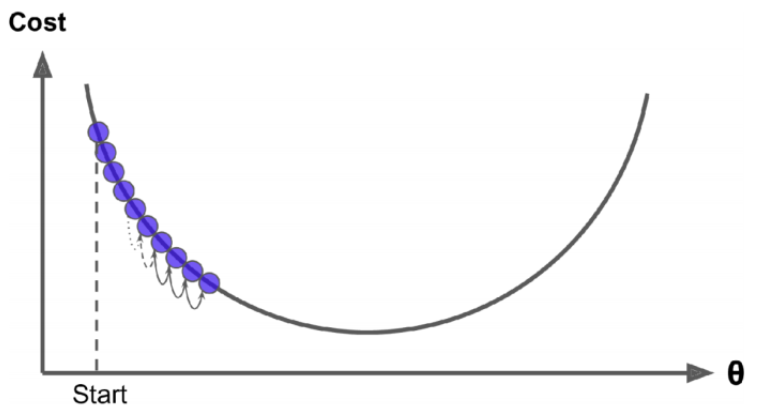
\includegraphics[width=\linewidth]{bilder/Learningrate_small(Geron).PNG}
		\caption{Zu kleine Learningrate}
		\label{abb: LearingrateSmall}
	\end{subfigure}	
	\begin{subfigure}[b]{0.32\linewidth}
		\centering
		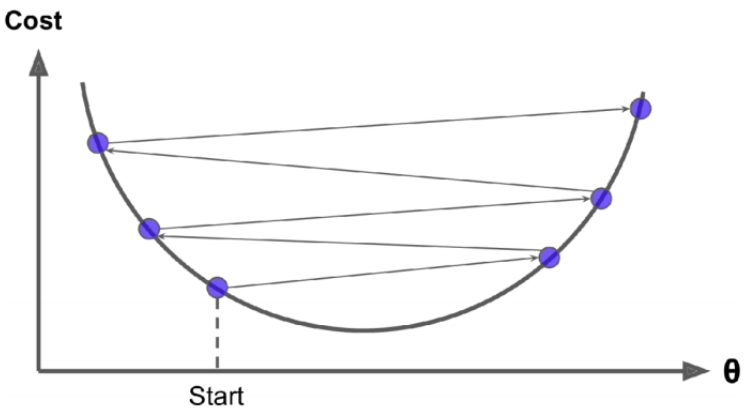
\includegraphics[width=\linewidth]{bilder/Learningrate_large(Geron).PNG}
		\caption{Zu große Learningrate}
		\label{abb: LearningrateLarge}
	\end{subfigure}
	\begin{subfigure}[b]{0.32 \linewidth}
		\centering
		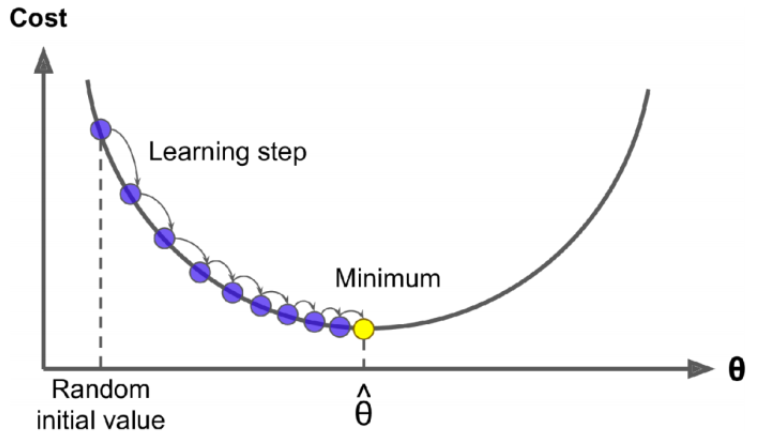
\includegraphics[width=\linewidth]{bilder/Learningrate_optimal(Geron).PNG}
		\caption{Optimale Learningrate}
		\label{abb: LearningrateOptimal}
	\end{subfigure}
	
	\caption{Visualisierung Learningrate}
\end{figure}

Nachdem der Lernprozess abgeschlossen wurde sind alle Gewichte fest und dürfen nicht mehr angepasst werden.
\cite{Goodfellow-et-al-2016}  \Todo{Referenzen}{}

Für die Validierung werden dann die Testdaten genutzt. Diese werden ebenfalls dem Netz als Input übergeben und klassifiziert. An dieser Stelle dürfen jedoch keine Anpassungen mehr vorgenommen werden, da der Lernprozess beendet ist. Für alle Testdaten werden die jeweiligen Fehlerraten bestimmt und ein gesamter Fehler z.B. über die Berechnung des Durchschnitts gebildet. Anhand dieses Fehlers kann die Genauigkeit der Klassifizierung des Netzes für fremde, vom Netz zuvor nicht gesehene Daten bestimmt werden.  \Todo{Referenzen}{}

Für die Validierung gibt es mehrere Ansätze, mit denen eine möglichst genaue Aussage über die Accuracy eines Intelligenten Systems getroffen werden kann. Zu diesen zählt zum Beipsiel Cross-Validation. Es ist jedoch auch möglich, mit je einem Trainings- und einem Testset das Netz zu validieren. \Todo{Referenzen}{}

\begin{definition}
	\label{def: CrossValidation}
	Cross-Validation
	
	Cross-Validation wird für das validieren von Trainingsergebnissen verwendet. Hierbei werden die vorhandenen Daten mehrfach in verschiedene Trainings- und Testsets (Mengen aus Trainings- und Testdaten) eingeteilt. Anschließend wird das Netz mit allen bestimmten Trainingssets trainiert und mit den zugehörigen Testsets validiert. Von den bestimmten Genauigkeitswerten wird anschließend der Durchschnitt als repräsentative Accuracy des Netzes berechnet. \cite{Basics-Training-Daten-ehler-CrossValidation}
\end{definition}

\section{Das gegebene Neuronale Netz}
\label{section: mein NN}
Das verwendete Neuronale Netz wurde bereits auf dem German Credit Datensatz trainiert zur Verfügung gestellt. Es besteht aus den folgenden fünf Schichten in der aufgezählten Reihenfolge: Linear, ReLU, Dropout, Linear und Softmax. 


Ein Linear Layer erhält den Namen aus der Funktion, die in den entsprechenden Knoten in diesem Layer als Aktivierungsfunktion verwendet wird. Es handelt sich hierbei somit um eine lineare Aktivierungsfunktion. \cite{Basics-Linear}
Knoten in einem ReLU Layer nutzen als Aktivierungsfunktion eine Rectifier Linear Unit Funktion. \cite{Basics-ReLU}
Der Dropout Layer wird genutzt, um Overfitting vorzubeugen. Dabei werden im Trainingsprozess zufällig Knoten der Schicht auf Null gesetzt, um so Informationen auszuschließen. \cite{Basics-Dropout}
Der Softmax Layer wird oft in Klassifikationsproblemen mit mehreren möglichen Ausgaben verwendet. Er bestimmt die Wahrscheinlichkeiten für alle Ausgabeknoten. Aus diesen wird dann derjenige mit der höchsten Wahrscheinlichkeit als Klassifizierung des Netzes ausgewählt. \cite{Basics-Softmax, Basics-Softmax-Hardware, Basics-Softmax-Hardware2}


\section{Ansätze}
\label{section: Methoden}
Die gewählten Ansätze entsprechen jeweils einem der in der Motivation erläuterten zum Öffnen der Black Box, die von komplexe Neuronale Netze gebildet wird. Eine Erklärung mithilfe von Surrogatmodellen passt zu der Idee der Modell-Erklärung. Counterfactuals entsprechen einer Erklärung der Entscheidung lediglich anhand der Ausgabe und sind damit Black Box Outcome Explanations. Der Ansatz der Erklärung durch die Bestimmung von Feature Contributions erklärt die innere Funktionalität des Netzes und bietet daher eine mögliche Lösung für das Black Box Inspection Problem. \cite{Guidotti}

Im folgenden wird die genaue Grundidee der drei Ansätze näher erläutert. In Kapitel 3 folgt zudem die Theorie und Implementierung für die konkreten Algorithmen.

\subsection{Surrogatmodelle}
\label{subsection: Surrogat}

Surrogatmodelle sind einfache, leicht interpretierbare, kostengünstige Approximationen von komplexen Funktionen. Ein solches Modell wird so trainiert, dass es genau wie die BlackBox-Funktion klassifiziert, inklusive der Fehler. Auf diese Weise können sie für Erklärungen von Black Box Funktionen genutzt werden. Bei der Approximation handelt es sich immer um ein leicht interpretierbares Modell, das sich weiterhin wie die zu erklärende Funktion verhält. \cite{InterpretableMLMolnar, TripathySurrogate}

Hierfür können alle interpretierbaren Modelle genutzt werden, zum Beispiel Entscheidungsbäume 
\cite{FrosstDecisionTree, TanSurrogate} oder lineare Modelle \Todo{Referenzen}{}. Für diese Arbeit werden genau diese beiden Methoden implementiert.

Welche Modelle tatsächlich als leicht interpretierbar eingestuft werden können ist jedoch eine subjektive Entscheidung. Im Allgemeinen können hierzu aber diejenigen Algorithmen gezählt werden, die zu einem gewissen Grad oder vollständig transparent sind. \cite{RudinStopExplaining} Die Aufstellung einer allgemeinen, alles umfassenden Definition für leicht interpretierbare Modelle ist nicht möglich, da je nach Anwendungsgebiet verschiedene Eigenschaften greifen. \cite{RudinStopExplaining}

Alle entsprechenden Modelle haben jedoch gemein, dass sie für einen Nutzer Sinn ergeben, sich also in einer für Menschen verständlichen Domäne befinden. \cite{MontavonLRP}


\subsection{Counterfactuals}
\label{subsection: CF}

Counterfactuals geben Erklärungen anhand von beispielhaften Änderungen gegeben und sind damit ein besipielbasierter Ansatz. \cite{InterpretableMLMolnar} Die Erklärung entsteht aus einer Wahl gut passender Attribute und einer Beschreibung der möglichen Wertänderung. Gut passend bedeutet hier, dass die Veränderung der Eigenschaften für das gesamte Objekt minimal ist, so wenig Eigenschaften, wie möglich gewählt werden und zugleich eine Änderung der Vorhergesagten Klasse erreicht wird. \cite{CangCounterfactuals}

Diese beispielhaften Erklärungen sind oftmals von folgender Form: Wäre Attribut $X=x_i$ und $Z=z_i$ gewesen, dann wäre die Entscheidung als $y_i$ anstelle von $y_j$ ausgefallen. Konkret könnte dies im Fall von Kreditwürdigkeit zu der Aussage \glqq Wäre das Einkommen in Höhe von $x_i= 5000$ \euro monatlich und die Schulden nicht höher als $z_i = 10000$ \euro gewesen, dann wäre die Kreditwürdigkeit als hoch genug eingestuft worden ($y_i = $ Kredit wird bewilligt statt $y_j = $ Kredit wird abgelehnt)\grqq. 

Auf diese Weise ist es möglich, ausschlaggebende Input-Features, sowie Handlungshinweise und Ähnliches bereitzustellen. Counterfactuals können so einen Einblick in die für eine Entscheidung wichtigen Eigenschaften liefern und zugleich Probleme bei der Entscheidungsfindung aufdecken. \cite{WachterCounterfactuals}

\subsection{Feature Contribution}
\label{subsection: Contribution}

Die Erklärung durch das bestimmen von Feature Contributions beschreibt einen Ansatz, bei dem der Beitrag einzelner Komponenten des Modells zu einer Klassifizierung betrachtet wird.  \cite{StrumbeljFeatureContribution, PalczewskaFeatureContribution} Hierfür wird anhand der Input-Features eine Erklärung bestimmt, die Wichtigkeit einzelner Eigenschaften für eine Entscheidung und somit den Beitrag dieser Inputs für das Ergebnis errechnet. \cite{} \Todo{Referenzen}{}

Auf diese Weise ist es möglich, auch einen Einblick in die inneren Schichten des Modells zu geben, da Contributions nicht nur auf die Input-Schicht beschränkt sein müssen. So kann mehr Transparenz geschaffen und die Funktionsweise der Black Box Funktion verständlich gemacht werden. Auch dieser Ansatz ermöglicht zudem das Erkennen möglicher Probleme des Modells anhand der bestimmten Wichtigkeiten für die Entscheidung. \cite{} \Todo{Referenzen}{}

Der Unterschied zu den vorherigen Ansätzen ist hier, dass auch alle inneren Schichten des neuronalen Netzes, die hidden layer, Teil der Erklärung sind. Das Verständnis wird nicht, wie bei Counterfactuals ausschließlich aus Ein- und Ausgaben bestimmt und hat im Gegensatz zur Erstellung vollständig neuer Modelle wie bei der Verwendung von Surrogatmodellen direkten Bezug zur zugrundeliegenden Funktion. \cite{}  \Todo{Referenzen}{}

Zu Algorithmen für diesen Ansatz gehören zum Beispiel die Layerwise Relevance Propagation (LRP) \cite{MontavonLRP} oder eine Kombination aus Shapley Values und dem deep LIFT Verfahren durch DeepSHAP. \cite{} \Todo{Referenzen}{}